\documentclass[12pt, letterpaper]{article}
\usepackage[utf8]{inputenc}
\usepackage[spanish]{babel}
\usepackage{amsmath, amssymb, amsthm}
\usepackage{graphicx}
\usepackage{array}
\usepackage{hyperref}
\usepackage{enumitem}
\usepackage{float}
\usepackage{minted}
\usepackage{xcolor}
\usepackage{booktabs}
\definecolor{lightgray}{rgb}{0.95,0.95,0.95}
%% Sets page size and margins
\usepackage[top=2.5cm,bottom=2.5cm,left=2cm,right=2cm]{geometry}
\usepackage{setspace}
\onehalfspacing
\usepackage{gensymb}
\usepackage{fancyhdr}
\pagestyle{fancy}
\fancyhead[L]{Compiladores}
\fancyhead[C]{Práctica 1}
\fancyhead[R]{Facultad de Ciencias UNAM}
\fancyfoot[C]{\thepage}
\renewcommand{\headrulewidth}{0.4pt}
\renewcommand{\footrulewidth}{0.4pt}

\begin{document}
\begin{titlepage}
    \centering
    \vspace{2cm}
    {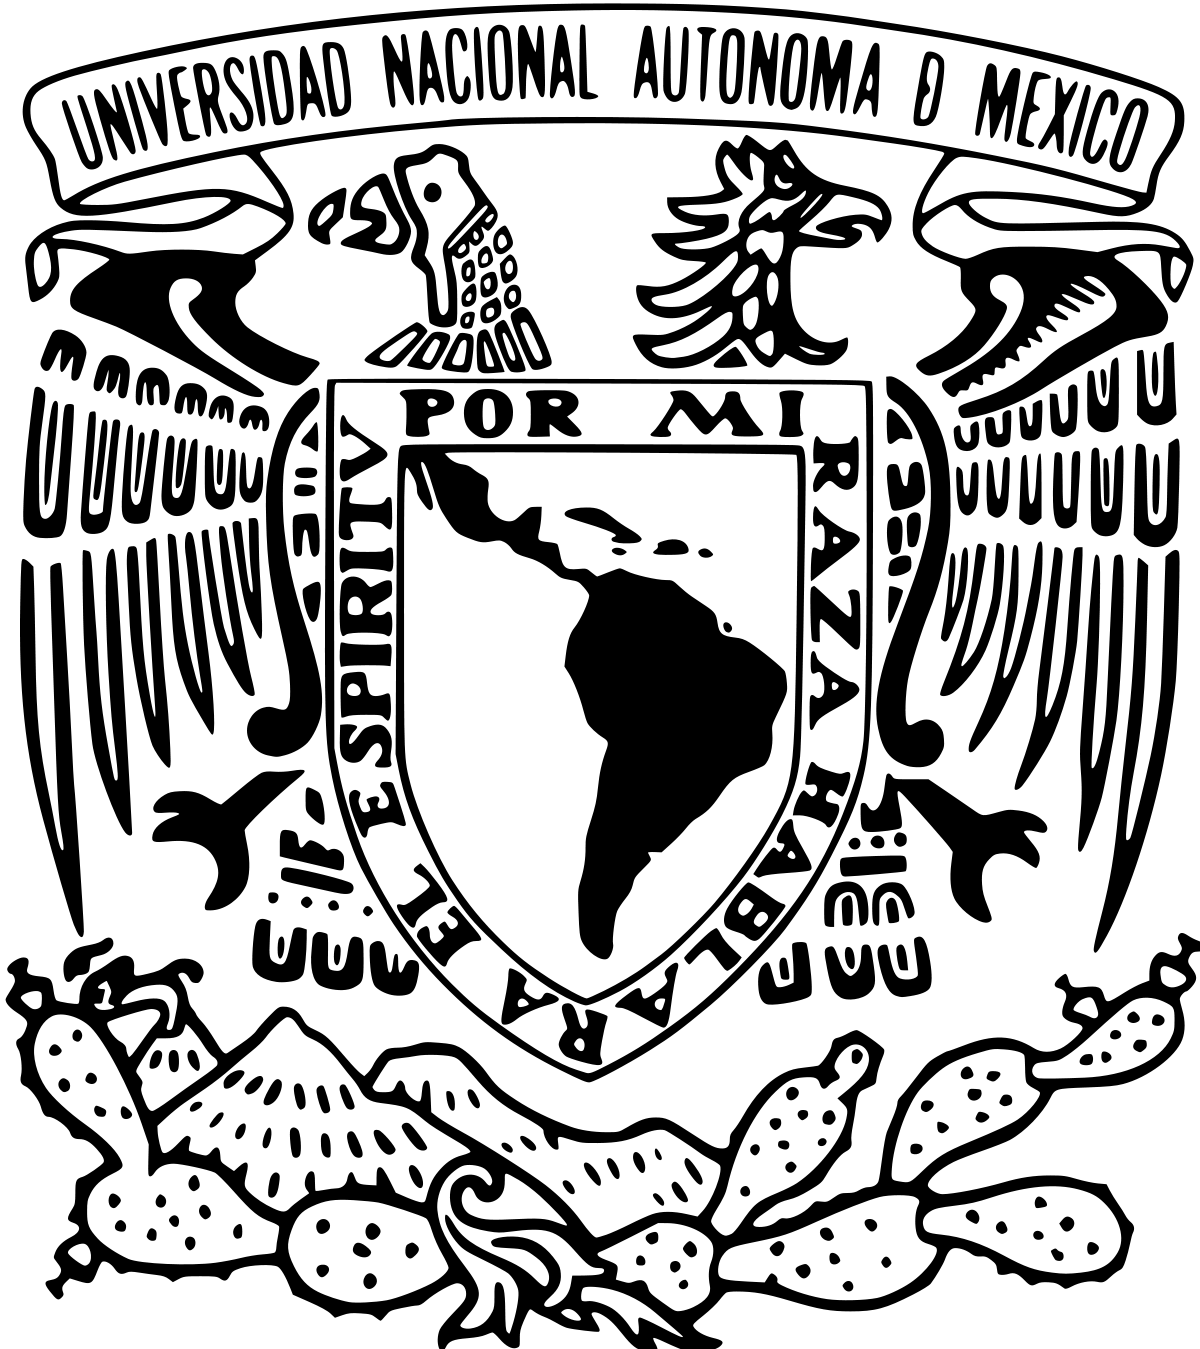
\includegraphics[height=3.2cm]{images/Logo_UNAM.png}}
    \hfill
    {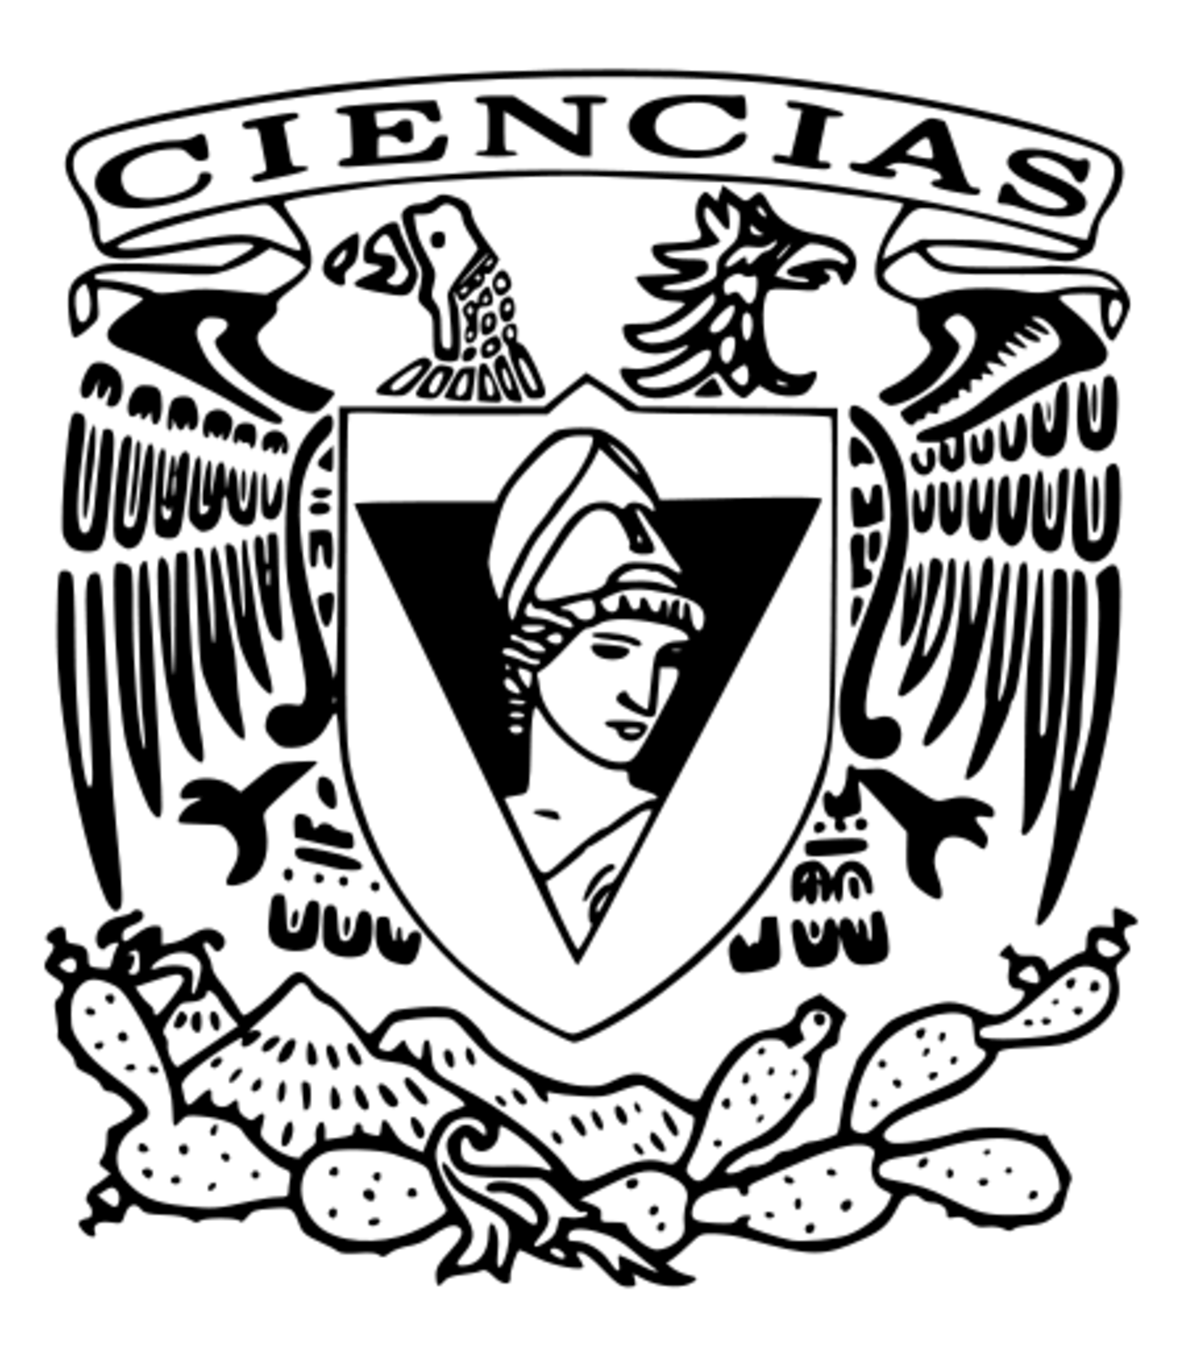
\includegraphics[height=3.2cm]{images/Logo_FC.png}\par}
    \vspace{0.5cm}
    {\scshape\LARGE \textbf{UNIVERSIDAD NACIONAL AUTÓNOMA DE MÉXICO} \par}
    \vspace{0.5cm}
    {\scshape\LARGE FACULTAD DE CIENCIAS \par}
    {\scshape\Large Ciencias de la Computación \par}
    \vspace{0.5cm}
    {\scshape\Huge Compiladores \par}
    {\scshape\Huge Semestre 2027-1 \par}
    \vspace{0.8cm}
    {\scshape\Huge \textbf{Práctica 1} \par}
    {\scshape\Huge \textbf{Regex a NFA} \par}
    \vspace{0.8cm}
    {\Large Integrantes: \par}
    \vspace{0.5cm}
    \noindent\begin{tabular}{p{10cm}p{3.5cm}}
    \toprule
    \Large
    Escobar Gonzalez Isaac Giovani & \Large 321336400 \\
    \Large
    Garduño Escobar Kevin Jonathan & \Large 321070629 \\
    \Large
    González Gutiérrez Antonio Tonatiuh & \Large 321195476 \\
    \Large
    Zaldivar Alanis Rodrigo & \Large 424029605 \\
    \bottomrule
    \end{tabular}\\
    \vspace{0.8cm}
    {\itshape\Large Fecha de entrega: 10 de Septiembre de 2026 \par}
\end{titlepage}

\subsection*{Validación:}
\subsection*{Descripción de la implementación}
\textbf{Nfa:} Para la construcción de los nfa, se optó por el enfoque orientado a objetos y modelar sus propiedades. Se creó un tipo struct nfa en el que los estados de estos están representados por números enteros, típicamente enumerados del cero (es el estado de inicio) al número de estados totales del nfa menos uno, que es el estado de aceptación. Aunque realmente, nfa solo da acceso a los estados de inicio y el de aceptación. Los demás estados son alcanzados mediante la lista de transiciones, un arreglo de structs de transicion que guardan estado origen, estado destino y el caracter que se lee para la transición. En la implementación, este arreglo es realmente un apuntador al inicio de la memoria.\\
Nuestra implementación del algoritmo de Ken Thompson para construir un nfa dada una expresión regex en notación post-fija, consiste en crear un arreglo de nfas (Lo creamos del tamaño de la expresión regex para asegurarnos de que sea suficiente y realmente se le da uso de pila). Posteriormente, procedemos a leer la regex postfija. Si encuentra un símbolo plano, no operador, se crea un autómata simple de dos estados que tiene una transición entre estos dos con el símbolo y se inserta en la pila. En caso de leer un operador binario, se obtienen los dos nfas en el tope de la pila y se construye uno nuevo.\\
Se hace un renombramiento de los estados de los nfas (particularmente de los estados de aceptación e inicio de los autómatas recibidos, y en las listas de transiciones) mediante un desplazamiento numérico basado en el número de nuevos estados, y, en el caso de la concatenación, basado en el tamaño del autómata prefijo. Análogamente para operadores unarios, se extrae el autómata en el tope de la pila. Cabe notar que para crear un nuevo autómata que recibe otro(s) y es/son operados por una operación, este autómata, así como su lista de transiciones, son creados en memoria desde cero y copian los valores de los autómatas según sea el caso y finalmente, una vez copiado lo que se necesitaba de los autómatas operandos, se liberan estos del espacio de memoria mediante la función nfa\_free. Además, si por alguna razón, falla la creación de alguna lista de transición, se regresa el autómata en estado de error también.
\begin{itemize}
    \item Unión: Se crea un nuevo estado final y uno inicial. Se crea una transición épsilon del estado inicial del nuevo autómata al estado inicial de cada uno de los nfas a unir. Análogamente, se crea una transición de cada estado de aceptación de los parámetros al nuevo estado de aceptación del autómata.
    \item Concatenación: Se crea una épsilon transición del estado de aceptación del autómata a al estado de inicio del autómata b. El estado de inicio del autómata es el del autómata \textit{a} y el de aceptación es el del autómata \textit{b}.
    \item Estrella de Kleene: Se crea un nuevo estado de aceptación y un nuevo estado inicial. Creamos 4 épsilon transiciones: Del nuevo estado inicial al estado inicial de \textit{a}, del estado inicial al estado final, del estado final de \textit{a} al nuevo estado final y del estado final de \textit{a} al estado inicial de \textit{a}.
    \item Cerradura positiva: Se crea un nuevo estado de aceptación y un nuevo estado inicial. Creamos 3 épsilon transiciones: Del nuevo estado inicial al estado inicial de \textit{a}, del estado final de \textit{a} al nuevo estado final y del estado final de \textit{a} al estado inicial de \textit{a}.
    \item Interrogación: Se crea un nuevo estado de aceptación y un nuevo estado inicial. Creamos 3 épsilon transiciones: Del nuevo estado inicial al estado inicial de \textit{a}, del estado inicial al estado final y del estado final de \textit{a} al nuevo estado final.
\end{itemize}
Cuando se acaba de leer la regex, se regresa el autómata en el fondo de la pila si es el único elemento que queda en esto. En caso contrario, se devuelve un autómata en estado de error.
\subsection*{Dificultades encontradas}
Para la elaboración de nfas, uno de los principales obstáculos que se encontraron, fue el cómo hacer el algoritmo eficiente. Ya que si ya teníamos autómatas construidos, podríamos simplemente añadir estados y conectarlos con transiciones, dependiendo del símbolo leído. Sin embargo, dada la implementación y representación que elegimos, resultó más conveniente simplemente copiar las transiciones y ajustarlas. Ya que gracias a nuestra implementación, nos ahorramos tener en memoria todos y cada uno de los estados. Además, de que al tener direcciones de memoria contigua tanto para los nfa como para las transiciones, nos ahorramos el tener que reservar memoria por cada nodo o transición creada y no están dispersos.

\subsection*{Resultados obtenidos.}

\end{document}
